% \begin{figure*}[ht!]
%     \centering
%     \RawFloats
%     \begin{minipage}[t]{0.65\textwidth}
%     	\vspace{-20pt}
%         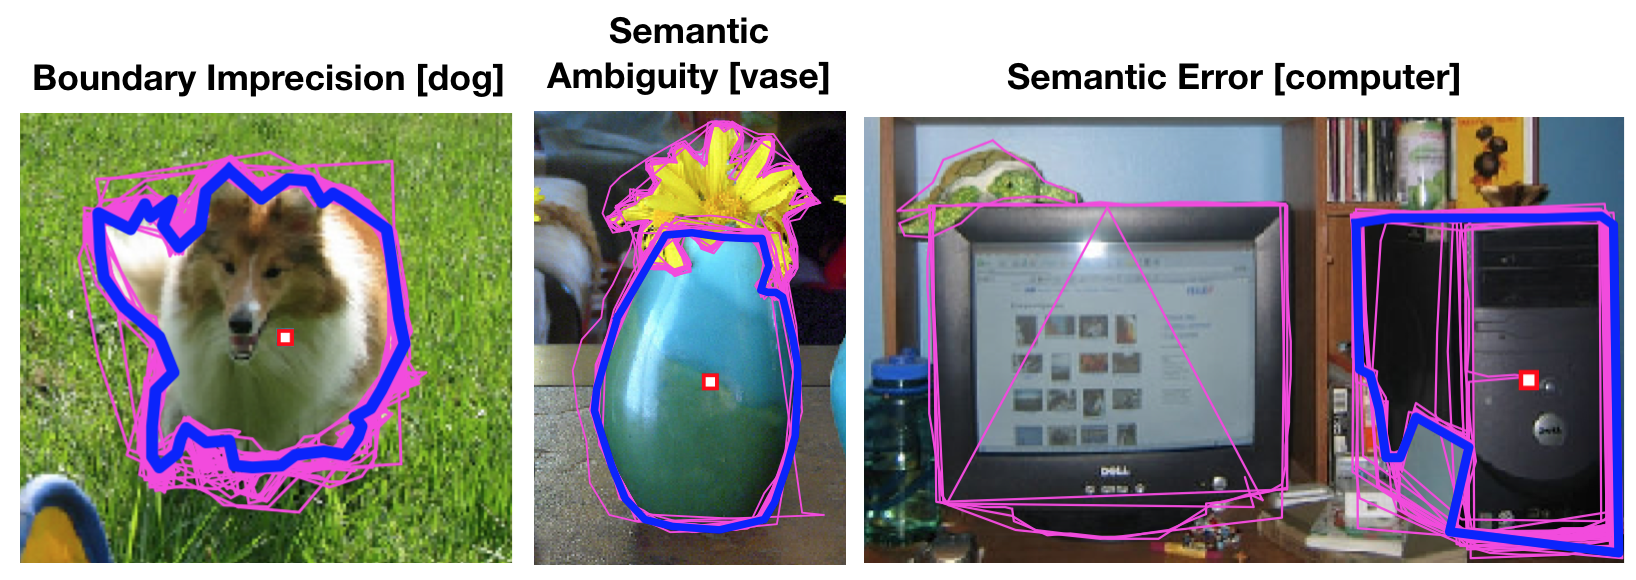
\includegraphics[width=\textwidth]{plots/error_examples.png} % second figure itself
%         \caption{Pink is the segmentation from individual workers. Blue solid line delineates the ground truth. The red boxed pointer indicates the task of interest shown to users.}
%         \vspace{-15pt}
%         \label{error_examples}
%     \end{minipage}
%     \begin{minipage}[t]{0.35\textwidth}
%     	\vspace{-25pt}
%         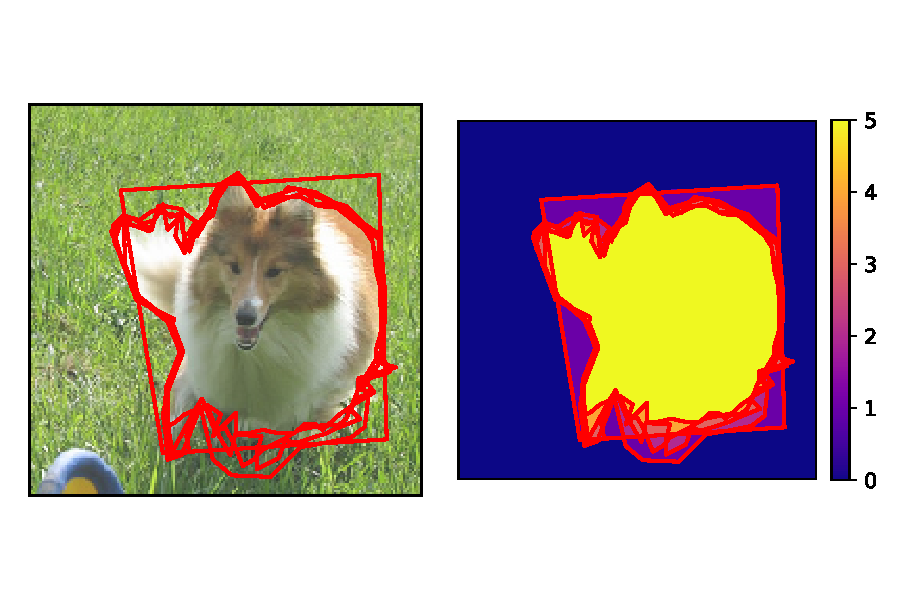
\includegraphics[width=\textwidth]{plots/tile_demo.pdf}
%         \vspace{-35pt}
%         \caption{Segmentation boundaries drawn by five workers in red. Right: Overlaid segmentation creates a masks where the color indicates the number of workers whose segmentation includes the tile region.}
%         \vspace{-20pt}
%         \label{tile_demo}
%     \end{minipage}\hfill
% \end{figure*}
\begin{figure}[h!]
    \centering
	\vspace{-20pt}
    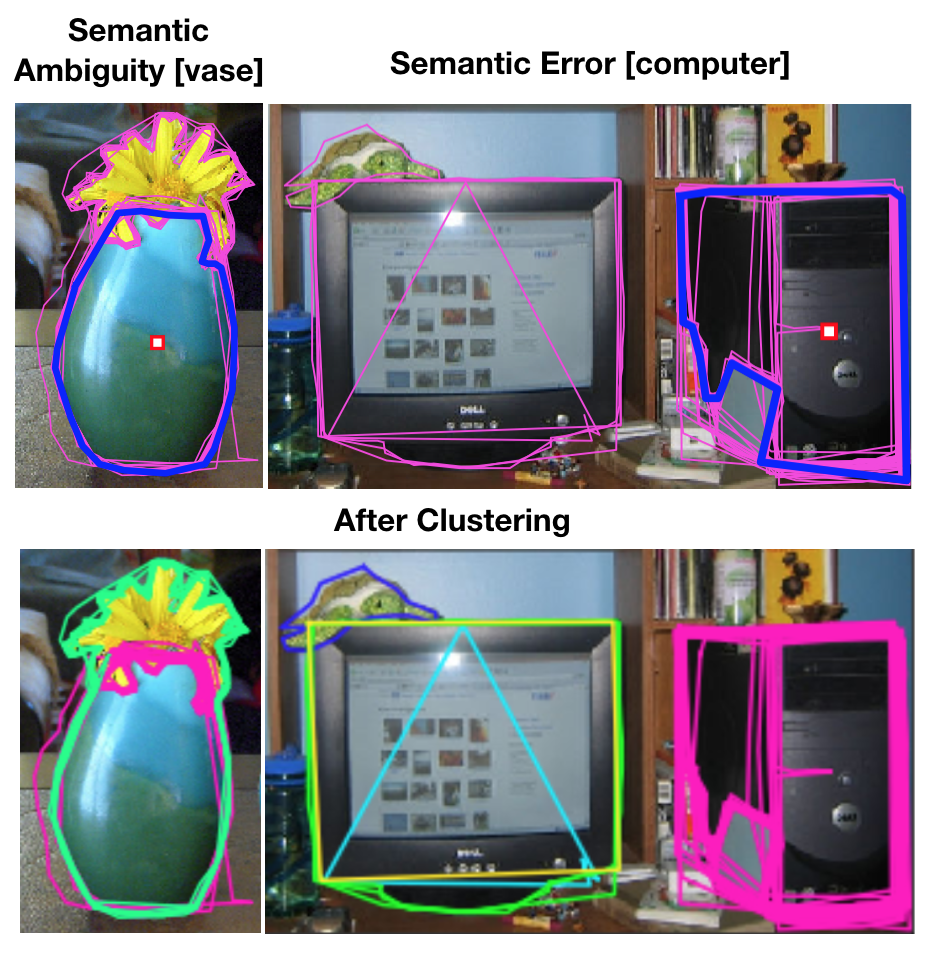
\includegraphics[width=\textwidth]{plots/semantic_error_clust.png}
    \caption{Top: Pink is the segmentation from individual workers. Blue solid line delineates the ground truth. The red boxed pointer is the interface icon indicating the semantic object to be segmented. Bottom: Boundary colors highlight different worker perspectives resulting from clustering.}
    \label{error_examples}
\end{figure}
\vspace{-10pt}
\section{Error Analysis}
\par Common worker errors can be classified into three types: (1) \textbf{Semantic Ambiguity:} differing opinions on whether particular regions belong to part of an object (Figure \ref{error_examples} Left); or (2) \textbf{Semantic Mistakes:} annotate the wrong object entirely (Figure \ref{error_examples} right); or (3) \textbf{Boundary Imprecision:} unintentional mistakes while drawing the boundaries, either due to low image resolution, small area of the object, or lack of drawing skills (Figure \ref{tile_demo} Left). In the following section, we will discuss a preprocessing method that we have developed to resolve semantic ambiguity and errors observed in prior work~\cite{Sorokin2008,Lin2014,Gurari2018}. Since quality evaluation in past literature have been largely focused on minimizing boundary precision issues, we will then describe novel aggregation-based algorithms that we have developed for this purpose and compare them with existing retrieval-based methods.% for addressing boundary imprecision. 
%\par %Out of the 46 objects in our dataset, 9 objects suffer from semantic ambiguity, 18 objects from semantic mistakes, and almost all objects suffer from some form of boundary imprecision to varying degrees. 
